\documentclass[paperwidth=160cm,paperheight=100cm,landscape,fontscale=0.3010]{baposter}
%Dortes fontscale: 0.2941
\usepackage{lipsum} 
%841mm x 1189mm
\usepackage[font=small,labelfont=bf,hypcap=false]{caption} % Required for specifying captions to tables and figures
%\usepackage{cite}
\usepackage{booktabs} % Horizontal rules in tables
\usepackage{relsize} % Used for making text smaller in some places
%\usepackage[urlcolor  = blue]{hyperref}
%\graphicspath{{figures/}} % Directory in which figures are stored
\usepackage{multicol}
%\usepackage[style=ieee]{biblatex}
%\addbibresource{bib.bib}
\usepackage[utf8]{inputenc} 
%\usepackage{hyperref}
\usepackage{placeins}
\usepackage{epstopdf}
\usepackage{subcaption}
\usepackage[]{graphicx}
\usepackage{natbib}
\usepackage{times}

\bibliographystyle{abbrvnat}

\selectcolormodel{RGB} %<-- Add colour model defintion
\definecolor{bordercol}{RGB}{255,255,255}%{33,26,82} % Border color of content boxes
\definecolor{headercol1}{RGB}{255,255,255}%{33,26,82} % Background color for the header in the content boxes (left side)
%\definecolor{headercol2}{RGB}{5,2,82} % Background color for the header in the content boxes (right side)
\definecolor{headerfontcol}{RGB}{0,0,0}%{255,255,255} % Text color for the header text in the content boxes
\definecolor{boxcolor}{RGB}{255,255,255} % Background color for the content in the content boxes

\begin{document}
\graphicspath{{Pictures/}}
\background{ % Set the background to an image (background.pdf)

}

\begin{poster}{
grid=false,
headerheight=0.17\textheight,
borderColor=bordercol, % Border color of content boxes
headerColorOne=headercol1, % Background color for the header in the content boxes (left side)
%headerColorTwo=headercol2, % Background color for the header in the content boxes (right side)
headerFontColor=headerfontcol, % Text color for the header text in the content boxes
boxColorOne=boxcolor, % Background color for the content in the content boxes
headershape=rectangle, % Specify the rounded corner in the content box headers
headershade=plain,
headerfont=\Large\sf\bf, % Font modifiers for the text in the content box headers
textborder=rectangle,
background=user,
headerborder=open, % Change to closed for a line under the content box headers
boxshade=plain,
eyecatcher=true
}
%
%----------------------------------------------------------------------------------------
%	TITLE AND AUTHOR NAME
%----------------------------------------------------------------------------------------
%
%\vspace{2em}
% Eye Catcher Images to go left of your title.
{

\includegraphics[height=0.13\textheight]{aau_logo_new.eps}
} %will not show if put eyecatcher=false
% Title
{\vspace{2pt}
Subjective Experience of Interacting with a Social Robot at a Danish Airport}
% Author
{
\vspace{3pt}
\normalsize{\textbf{Andreas Kornmaaler Hansen, Emil Bonnerup, Juliane Nilsson, Lucca Julie Nellemann \& Sara Nielsen}\\
Psychology Engineering - 17gr782 - Fall 2017 - School of Information and Communication Technology\\ Aalborg University, Aalborg, Denmark\\ }
$\{$akha12, ebonne14, jnils12, ljne14, snie14$\}$@student.aau.dk\\
}
{

\includegraphics[height=0.13\textheight]{aau_logo_new.eps}
}

%----------------------------------------------------------------------------------------
%	INTRODUCTION
%----------------------------------------------------------------------------------------
\headerbox{Introduction}
{name=introduction,column=0,row=0, span=1}
{\parskip 5pt   
This study originates from a social robot research project at Aalborg University with the aim of developing and implementing robots in a variety of contexts. This raises questions on how social robots should behave and which variables in a social robot is important. When important variables are eliciteted scales can be developed from these variables which can be use to test a social robot. The study consists of two tests, one where variables are elicitated and one where the scales are used to evaluate the robot. 
}

\headerbox{Method - Elicitation of words}
{name=method1,span=1,column=0,below=introduction, span=1}
{\parskip 5pt 
The first test was conducted on Danish travellers who interacted with a social robot in natural settings. The test was conducted at Aalborg Airport (AAL). The travellers who interacted with the robot were asked to participate in a semi-structured interview about their first impressions while being observed during both the interaction and the interview. 

\textbf{Materials}
For the test a \textit{Double} robot with an iPad Air 2 was used. The head mount was changed angeling the iPad upwards. The modified \textit{Double} robot is shown on figure 1. The \textit{Double} robot was remotely controlled via a computer and a present controller. On the screen a developed wireframe to help with wayfinding in AAL was presented. 
\vspace{-10pt}  

\begin{center}
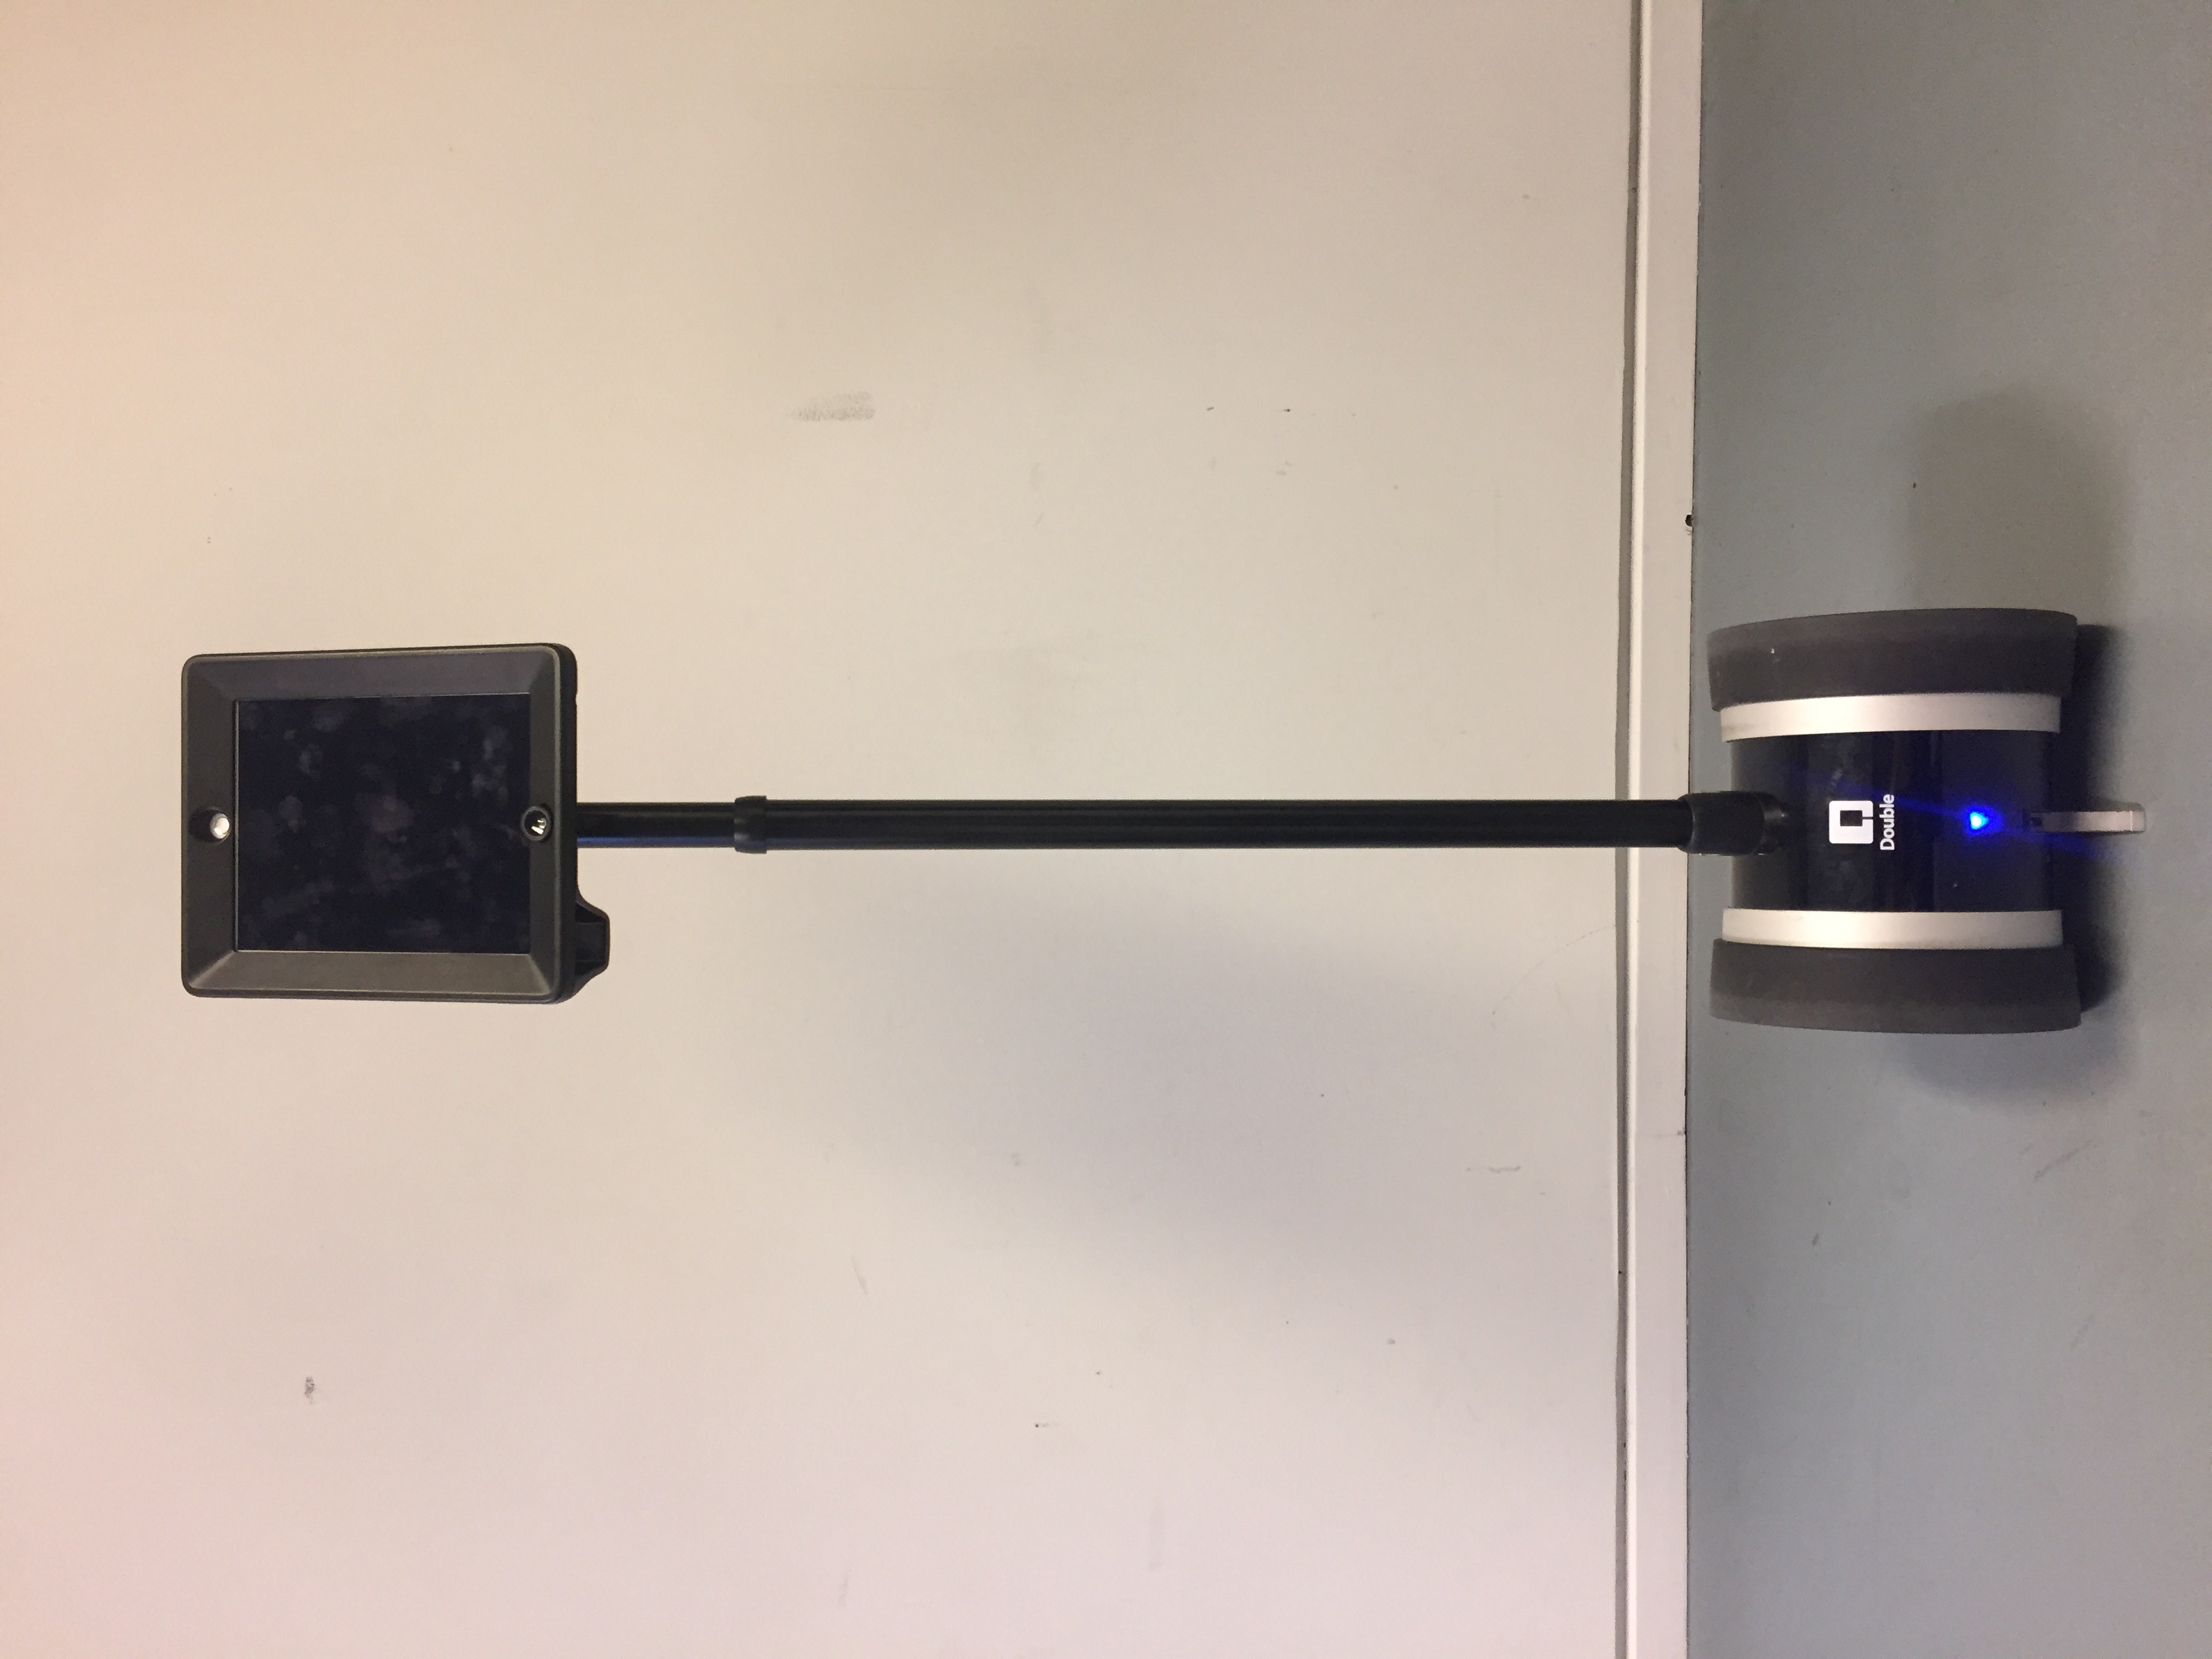
\includegraphics[width=0.30\linewidth]{ModificeretDoubleFront.eps}
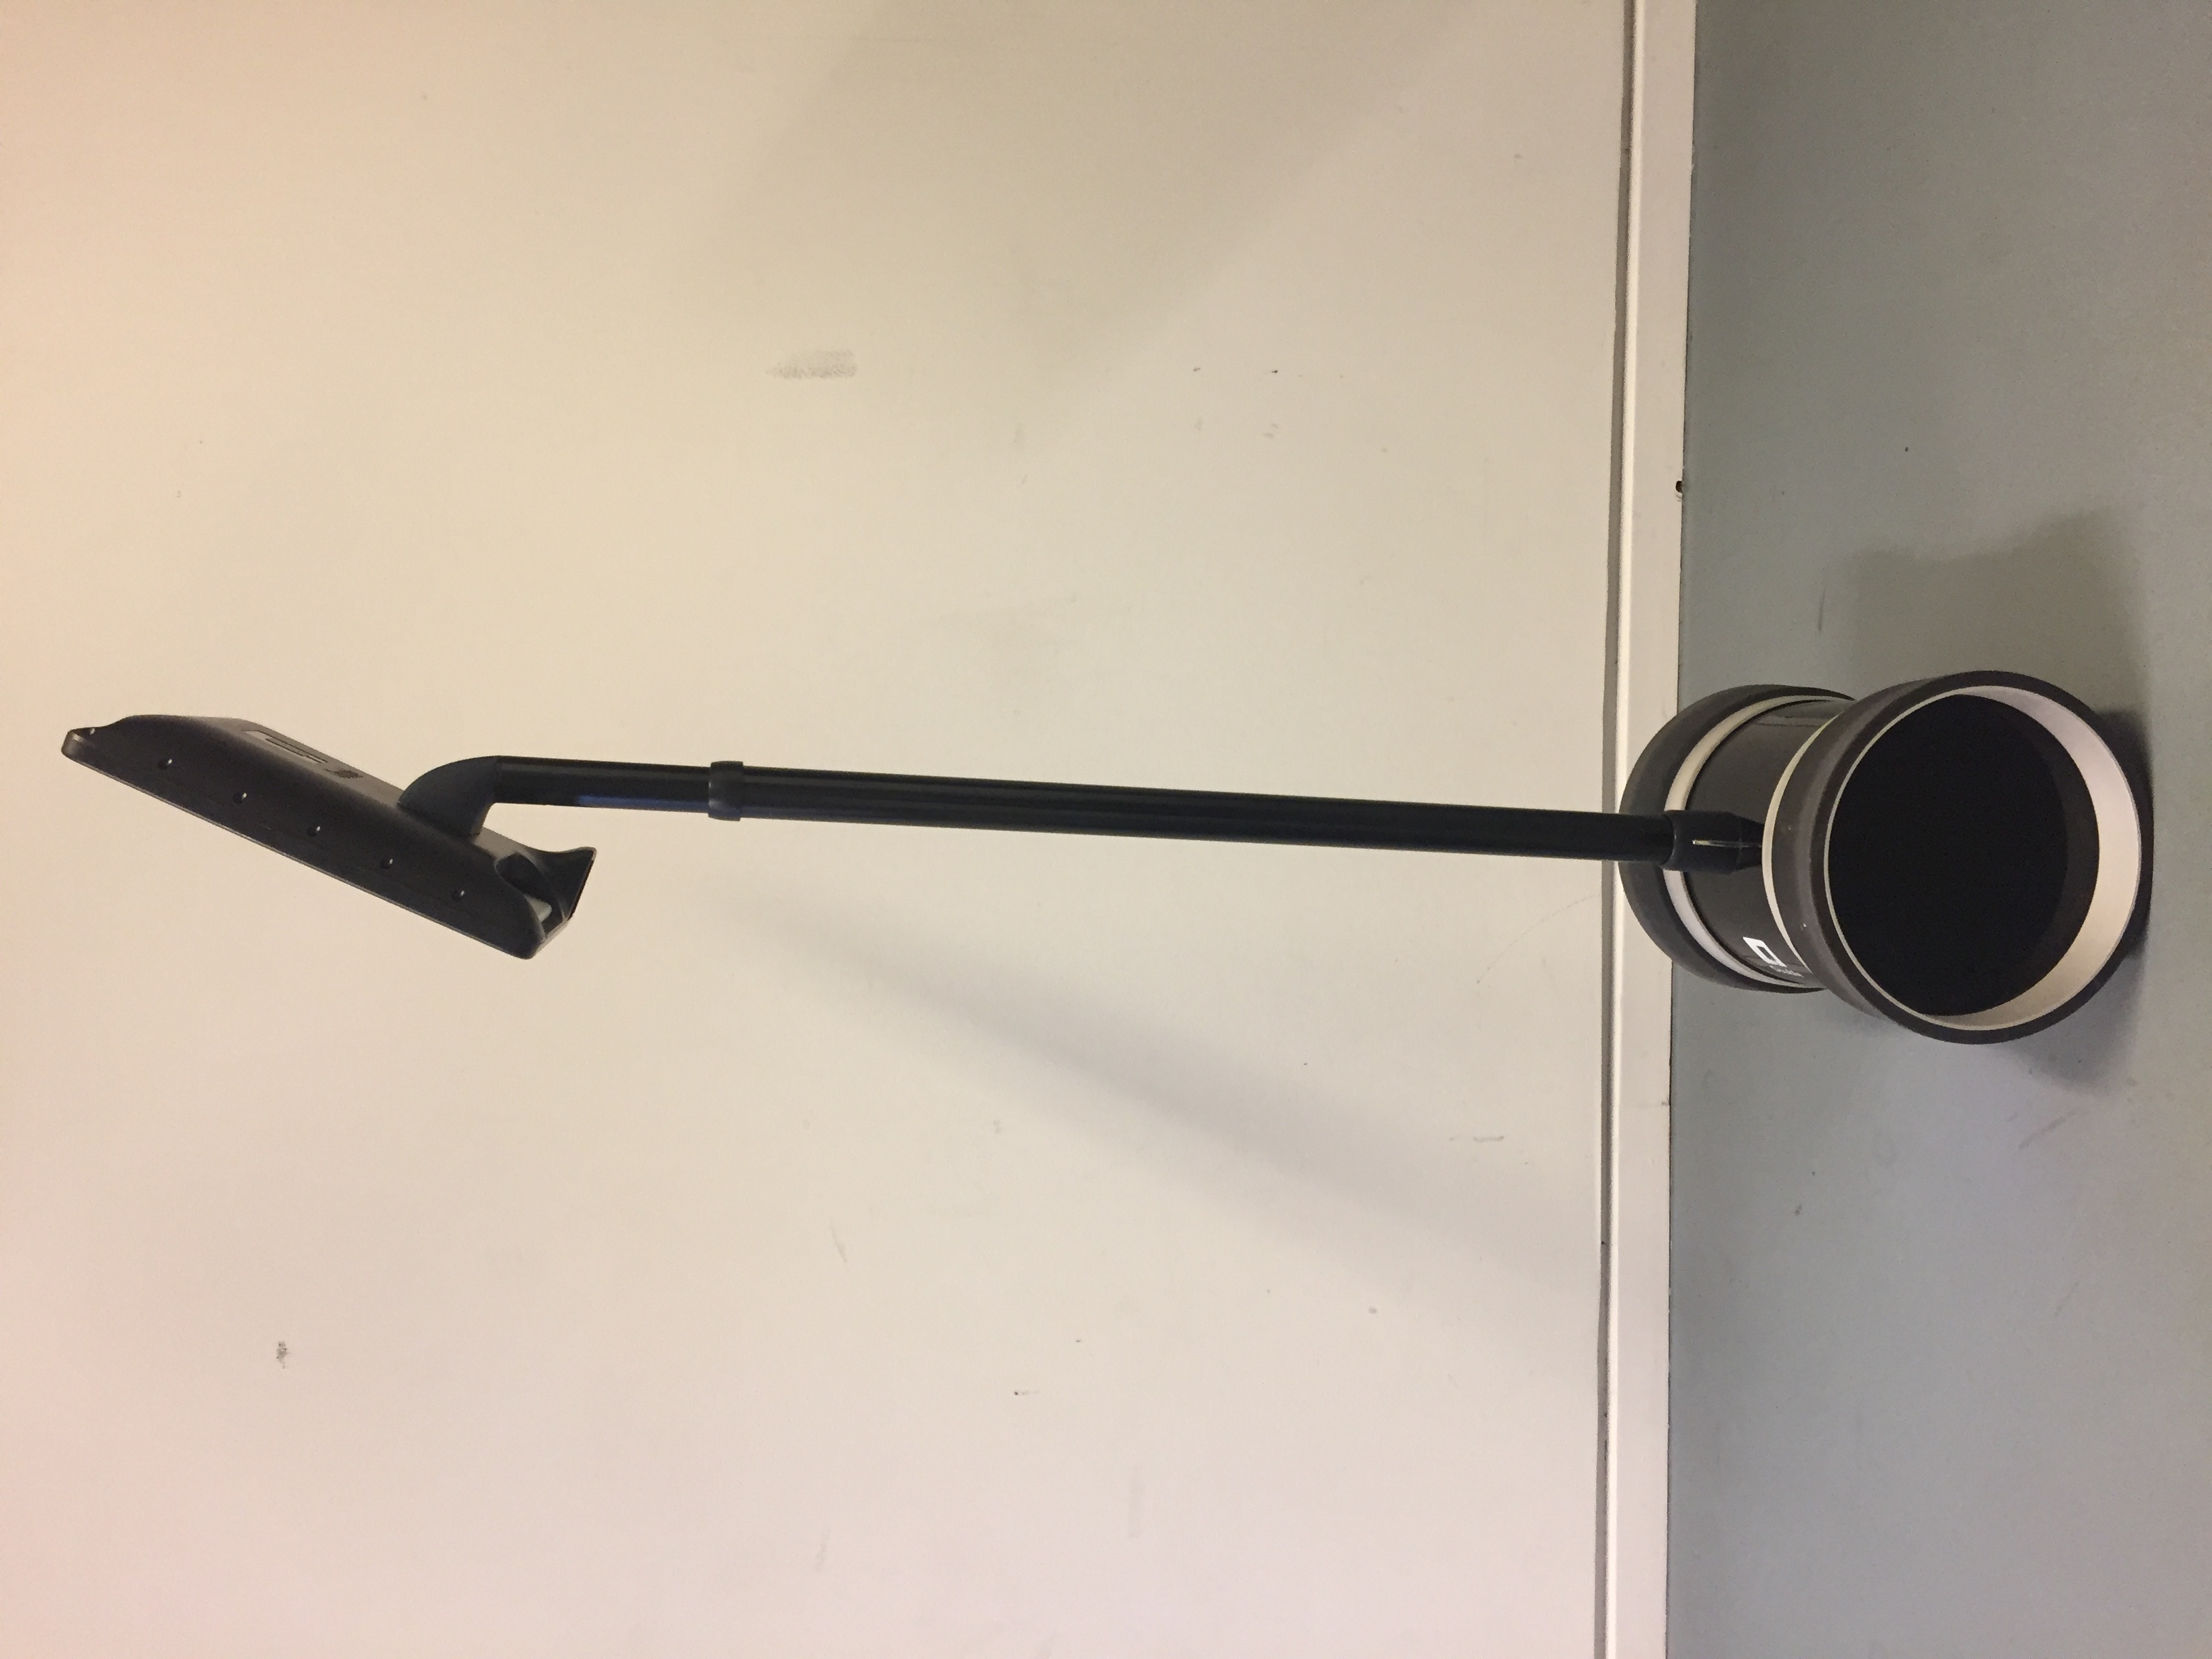
\includegraphics[width=0.30\linewidth]{ModificeretDoubleSide.eps}

\textbf{Figure~1. }\textit{Double}'s front and profile.
\end{center}
\vspace{-10pt}  

\textbf{Subject Recruitment}
16 females and 14 males with a mean age of 37.9 years (SD=17.1) participated. The subjects were recruited by the robot, because it provides a more ecological and undisturbed interaction between robot and subject. The robot approached potential subjects after the security check and asked to help travellers with wayfinding. If travellers wanted help, they were presented with four wayfinding options: Food, Shopping, Toilets or Gate information. After the interaction the robot led subjects to an interviewer. 

\textbf{Semi-structured Interview}
The interview was a two part interview. The first part consisted of probing the subjects for their first impression and experience of interacting with the robot in regard to their thoughts about the robot itself. Subjects were asked about their opinion regarding the robot's approach, relevance, and reliability. The second part consisted of asking questions relating to the robots physical characteristics such as speed, height, distance, movements, appearance, and approach. These questions were asked because the variables are known to affect the experience of HRI.

\textbf{Data Processing}
The interviews and observations were coded into affinity notes and an affinity diagram was made. This affinity diagram is pivotal in eliciting the variables that affect HRI, and thereafter in creating the scales to be used for further work. 
567 affinity notes were sorted into 10 green categories with individual subcategories. To gain more insight it was decided to mix the spontaneous answers from the conversation topics with the answers from the specific questions. These were not differentiated in the affinity diagram.
}


\headerbox{Results - Elicitation of words}
{name=results1,span=1,column=1,aligned=introduction, span=1}
{\parskip 5pt 

}


\headerbox{Method - Scale Testing}
{name=method2,span=1,column=1,below=results1}
{\parskip 5pt 


}

\headerbox{Results - Scale Testing}
{name=results2,span=1,column=2,aligned=introduction}
{\parskip 5pt


}


\headerbox{Conclusion}
{name=conclusion,span=1,column=3,aligned=introduction}
{\parskip 5pt

}


\headerbox{Acknowledgements}
{name=akn,span=1,column=3,below=conclusion}
{\parskip 5pt

}


\headerbox{References}
{name=references,column=3,below=akn}
{
\renewcommand{\section}[2]{}%
%\parskip 5pt
 %   \bibliography{bib.bib}
%\tiny
\footnotesize
%Dorte har skrevet kilder ind på følgende måde
%Abdala C (1996) JASA \textbf{100}(6):3726-3740.
%Bonfils P et al. (1991) \textit{Arch Otolaryngol Head Neck Surg} \textbf{117}(10):1167–1171.
%Brown DK et al. (2000) \textit{Hearing Res}. \textbf{145}(1-2):17-24.
}


%-------------------------------------------------------------------------

\end{poster}
\end{document}